\documentclass[main]{subfiles}


\title[Dynamic Approaches]{Dynamic Approaches}
\subtitle{Why Dynamic Optimization?}
\author[André Biedenkapp]{André Biedenkapp}
\date{}

\titlebackground*{images/AutoML_LearningToLearn2}

%\institute{}
%\date{}

\begin{document}
	
	\maketitle
%-----------------------------------------------------------------------
%----------------------------------------------------------------------
%-----------------------------------------------------------------------
%----------------------------------------------------------------------
\begin{frame}{Why Dynamic?} 

%\begin{itemize}
    %\item 
    We often treat AutoML as a black-box problem
    \pause
    \begin{columns}
    \column{0.33\textwidth}
        \centering
        \onslide<2->{
        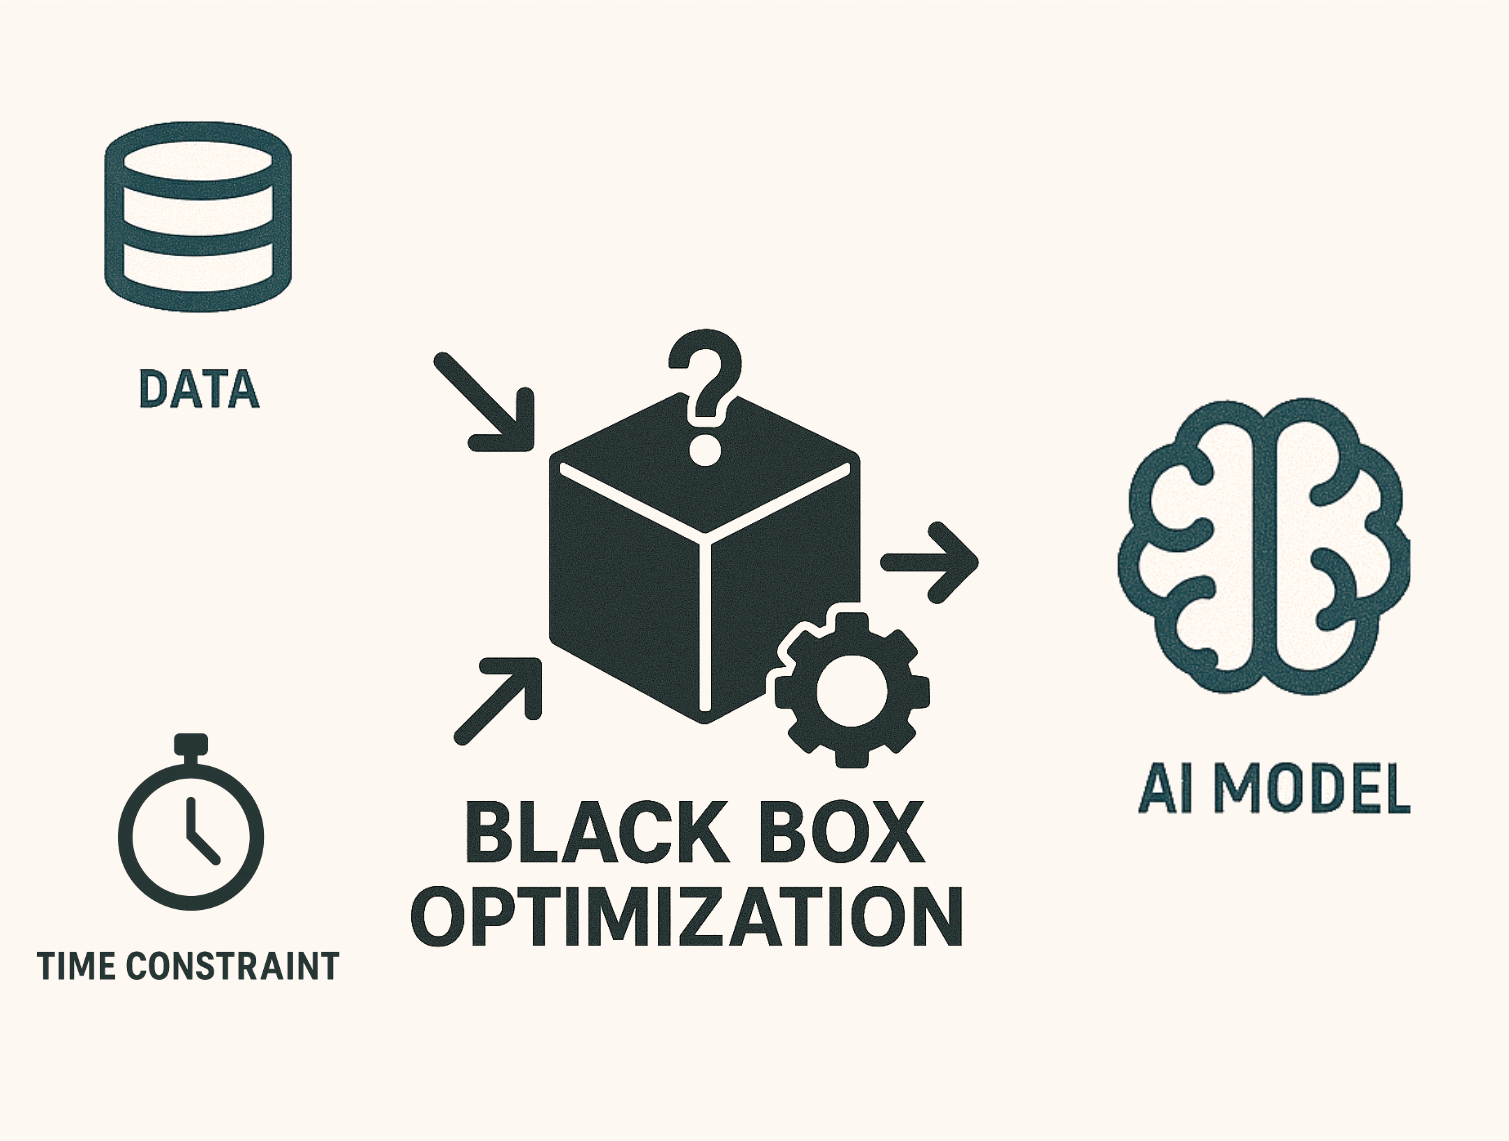
\includegraphics[width=1\textwidth]{images/interface_data_constraint_model.png}}
    \column{0.33\textwidth}
        \centering
        \onslide<3->{
        
\includegraphics[width=\linewidth]{images/interface_data_space_config.png}}
    \column{0.33\textwidth}
        \centering
        \onslide<4->{
        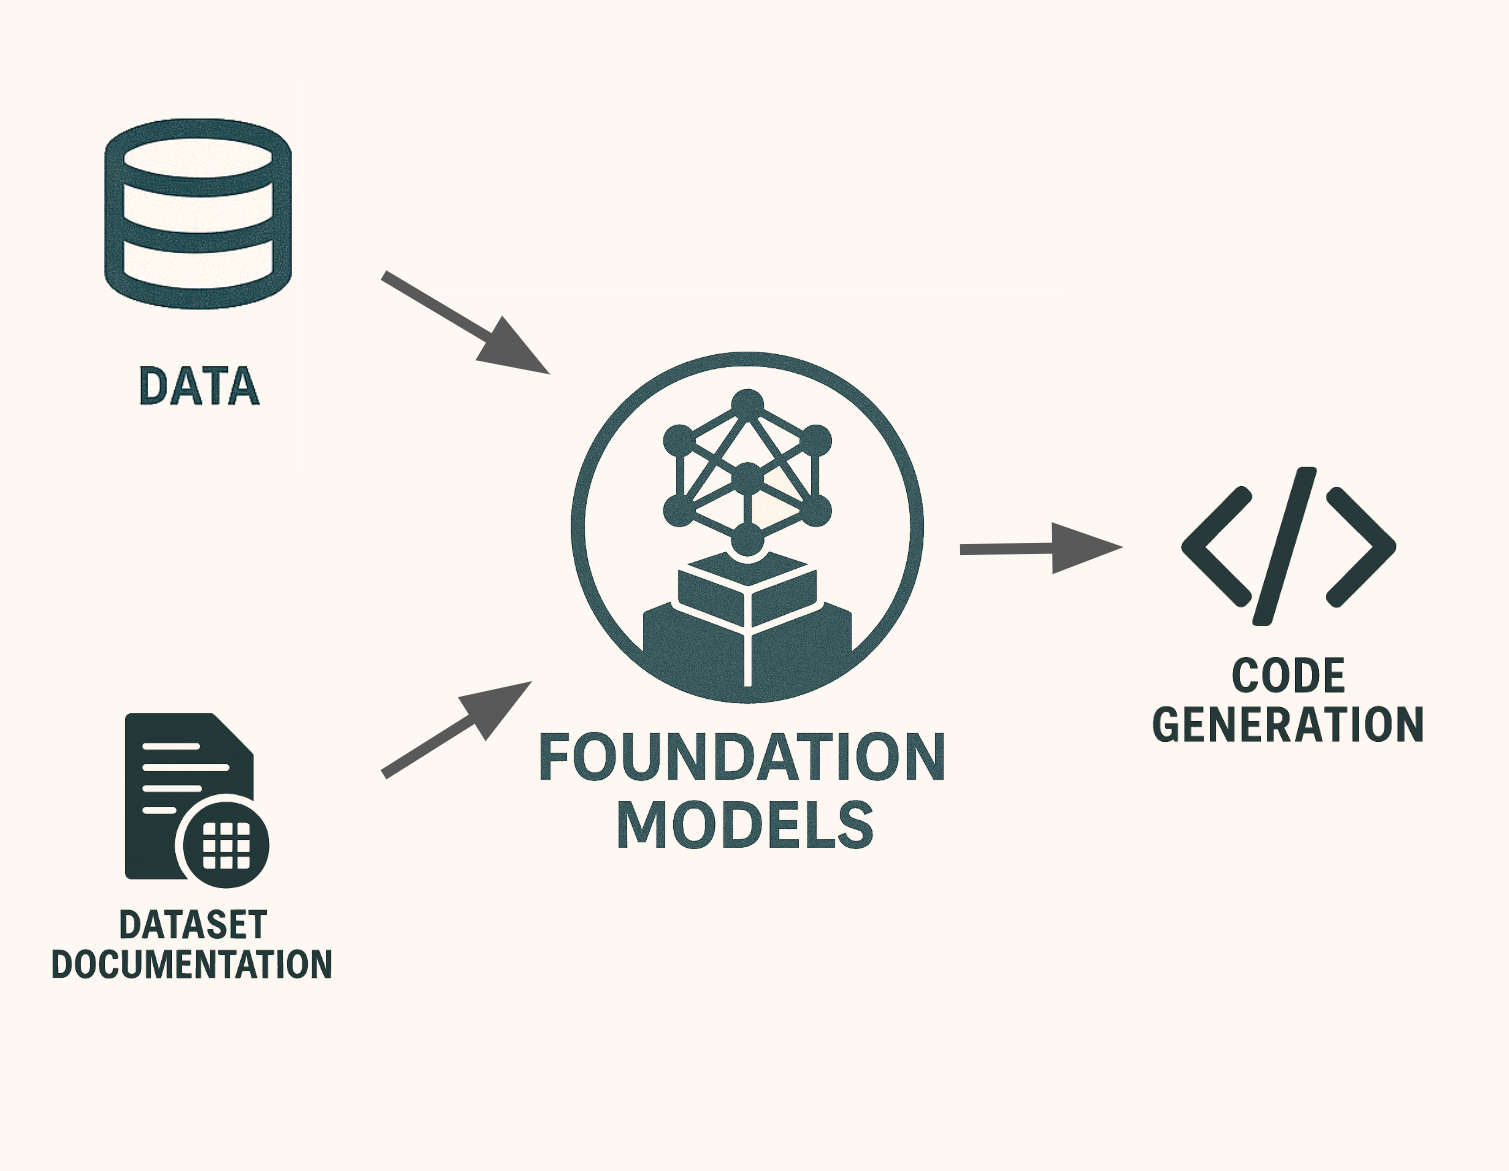
\includegraphics[width=\linewidth]{images/interface_data_docu_code.png}}
    \end{columns}
    \onslide<5->{
    We do not take into account what happens inside the box!}
    
%\end{itemize}

\end{frame}
%-----------------------------------------------------------------------
%----------------------------------------------------------------------
\begin{frame}{Why Dynamic?} 

   Many learning approaches are \emph{iterative}!
    \pause
    \begin{enumerate}
        \item Initialize model
    \pause
        \item Fit model to data
    \pause
        \item Observe performance / compute loss
    \pause
        \item Adapt model based on loss
    \pause
        \item Repeat 2 - 4 until learning budget is exhausted
    \end{enumerate}
    \pause
    \vspace{2ex}
    \begin{itemize}
        \item Learning explores/traverses a solution space
        \item Dynamic optimization can tackle {\color{red}non-stationary problems}
    \end{itemize}
\end{frame}
%-----------------------------------------------------------------------
%----------------------------------------------------------------------
\begin{frame}{Example: Learning Rates in Deep Learning}
    Update rule $\weights_{i+1} = \weights_{i} - \alpha\nabla\fh_{\weights_{i}}$ using learning rate $\alpha$ on a simple parabola
    \vspace{2ex}
    \begin{columns}
    \column{0.33\textwidth}
        \centering
        \only<2->{
        $\alpha$ too small:\\takes long to converge
        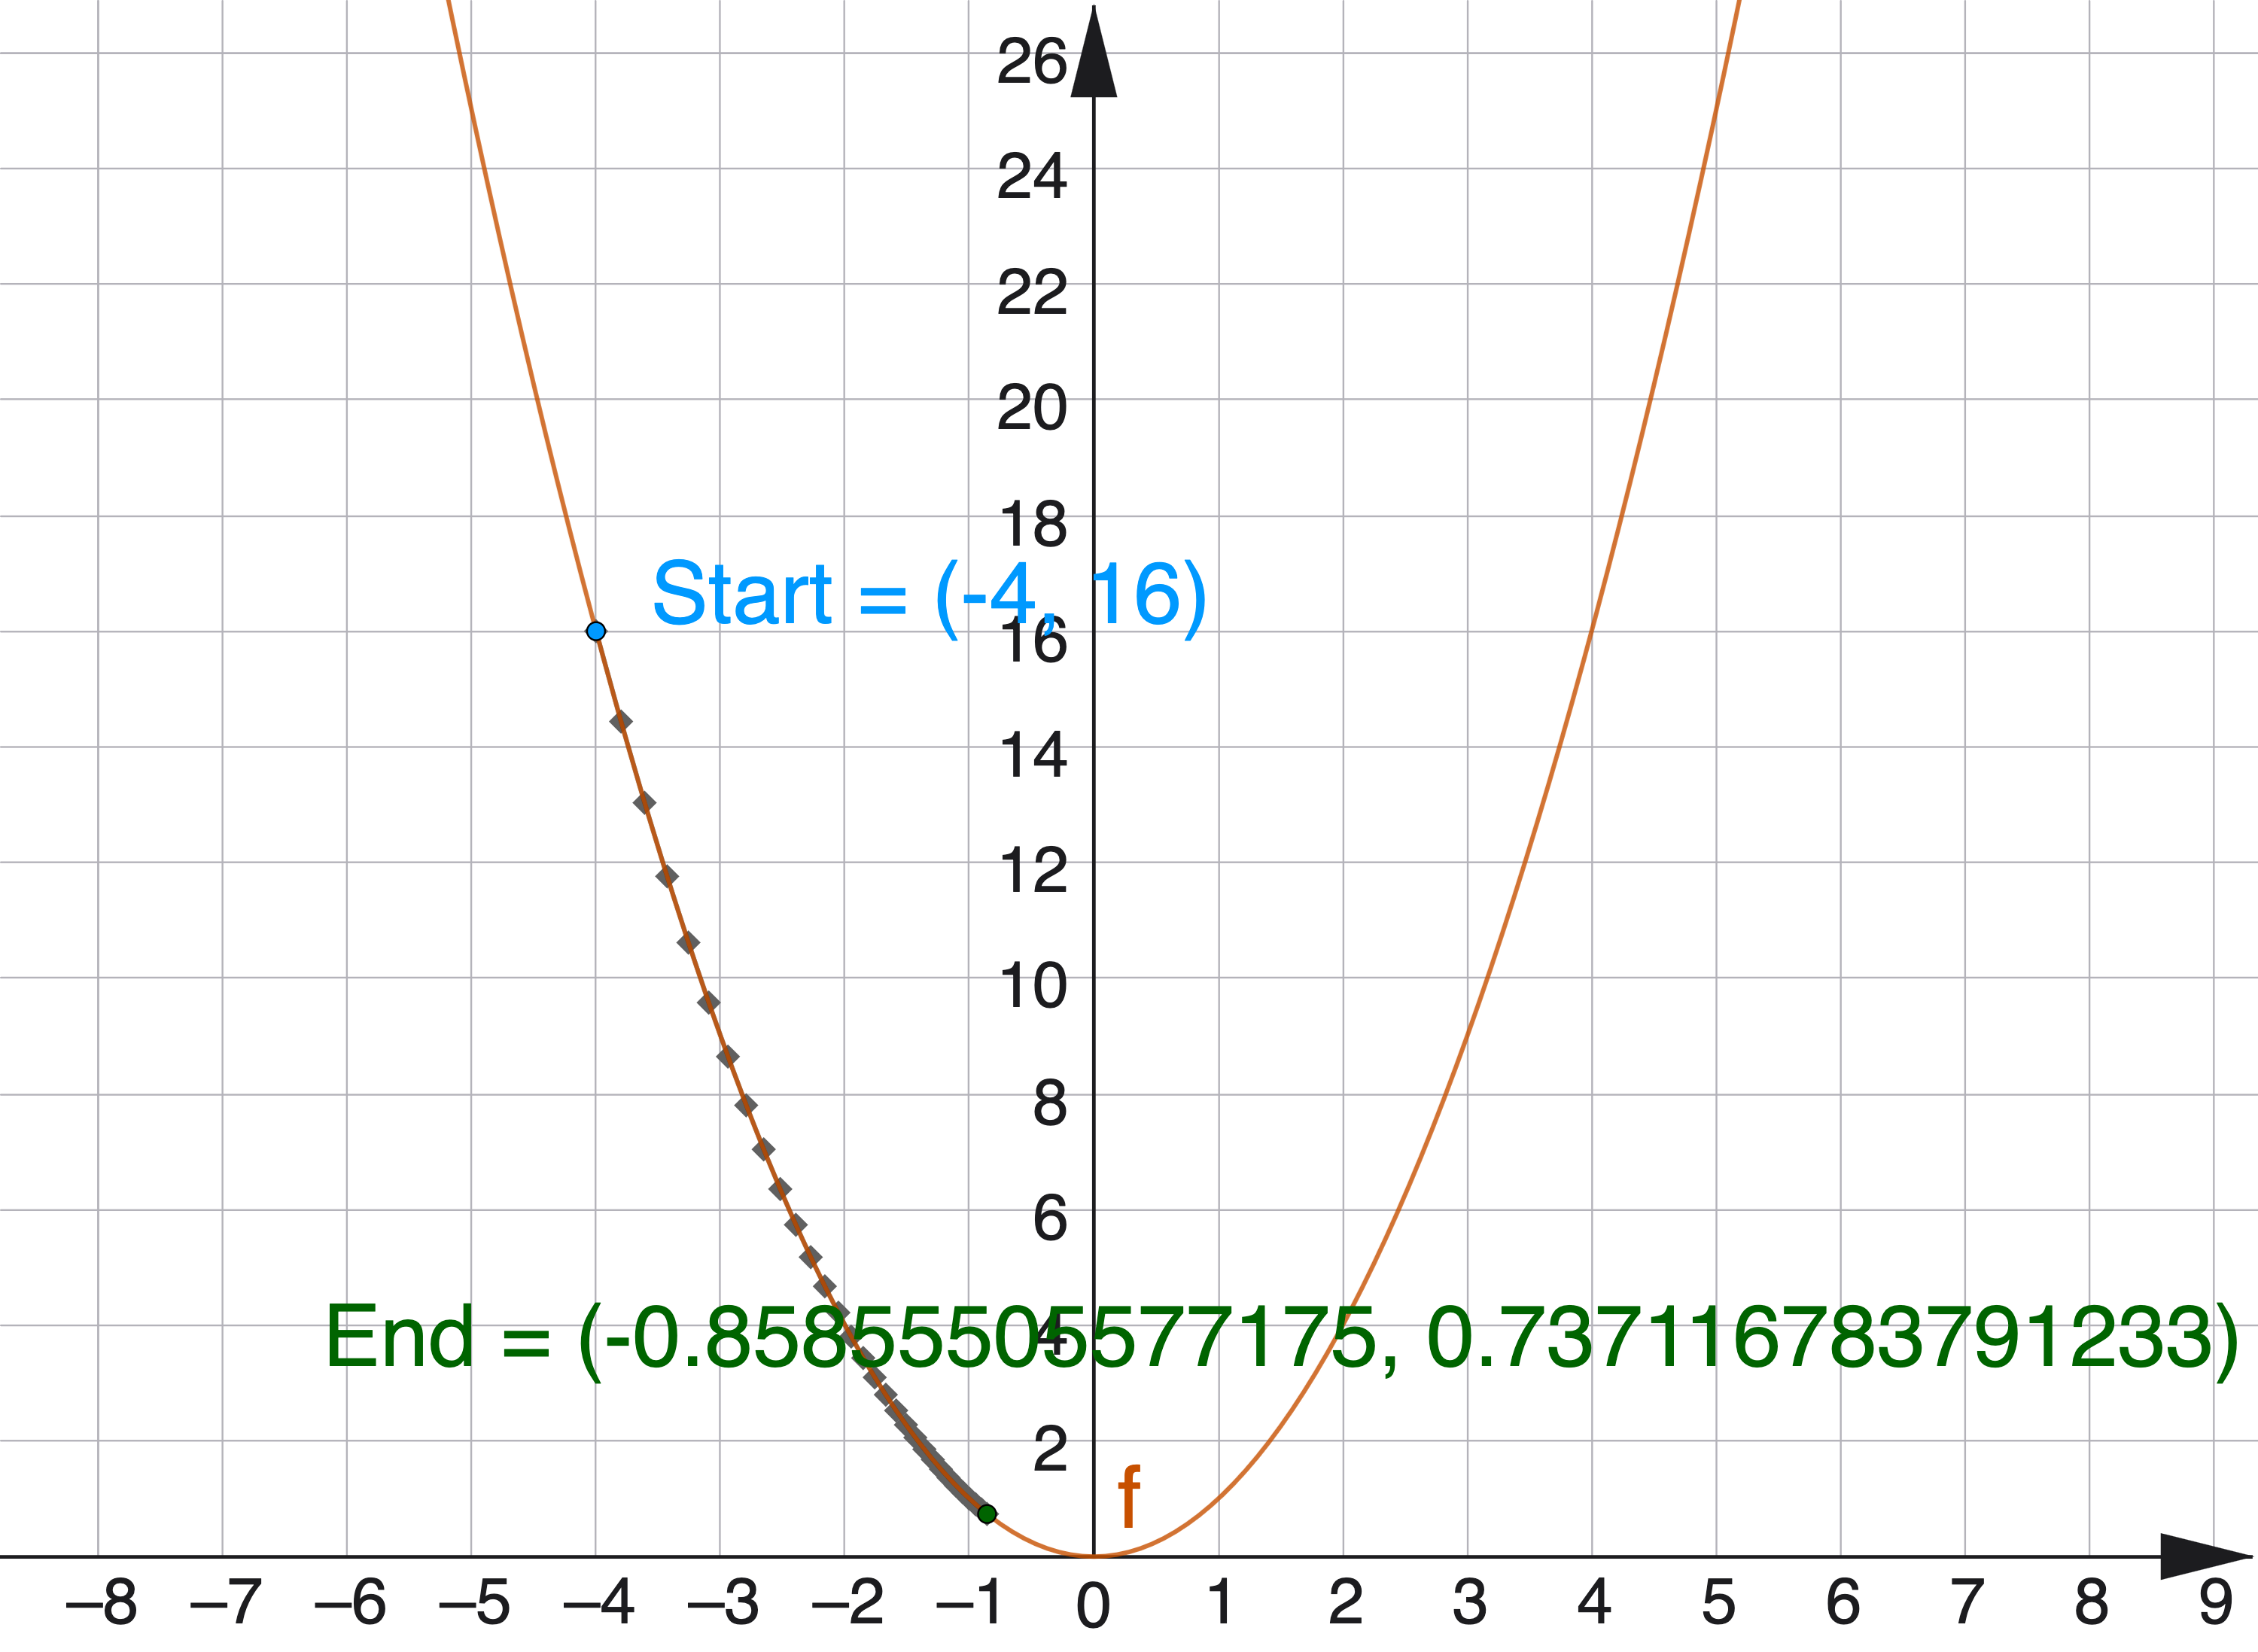
\includegraphics[width=\linewidth]{images/lr_too_small}}
    \column{0.33\textwidth}
        \centering
        \only<3->{
        $\alpha$ small enough:\\convergence
        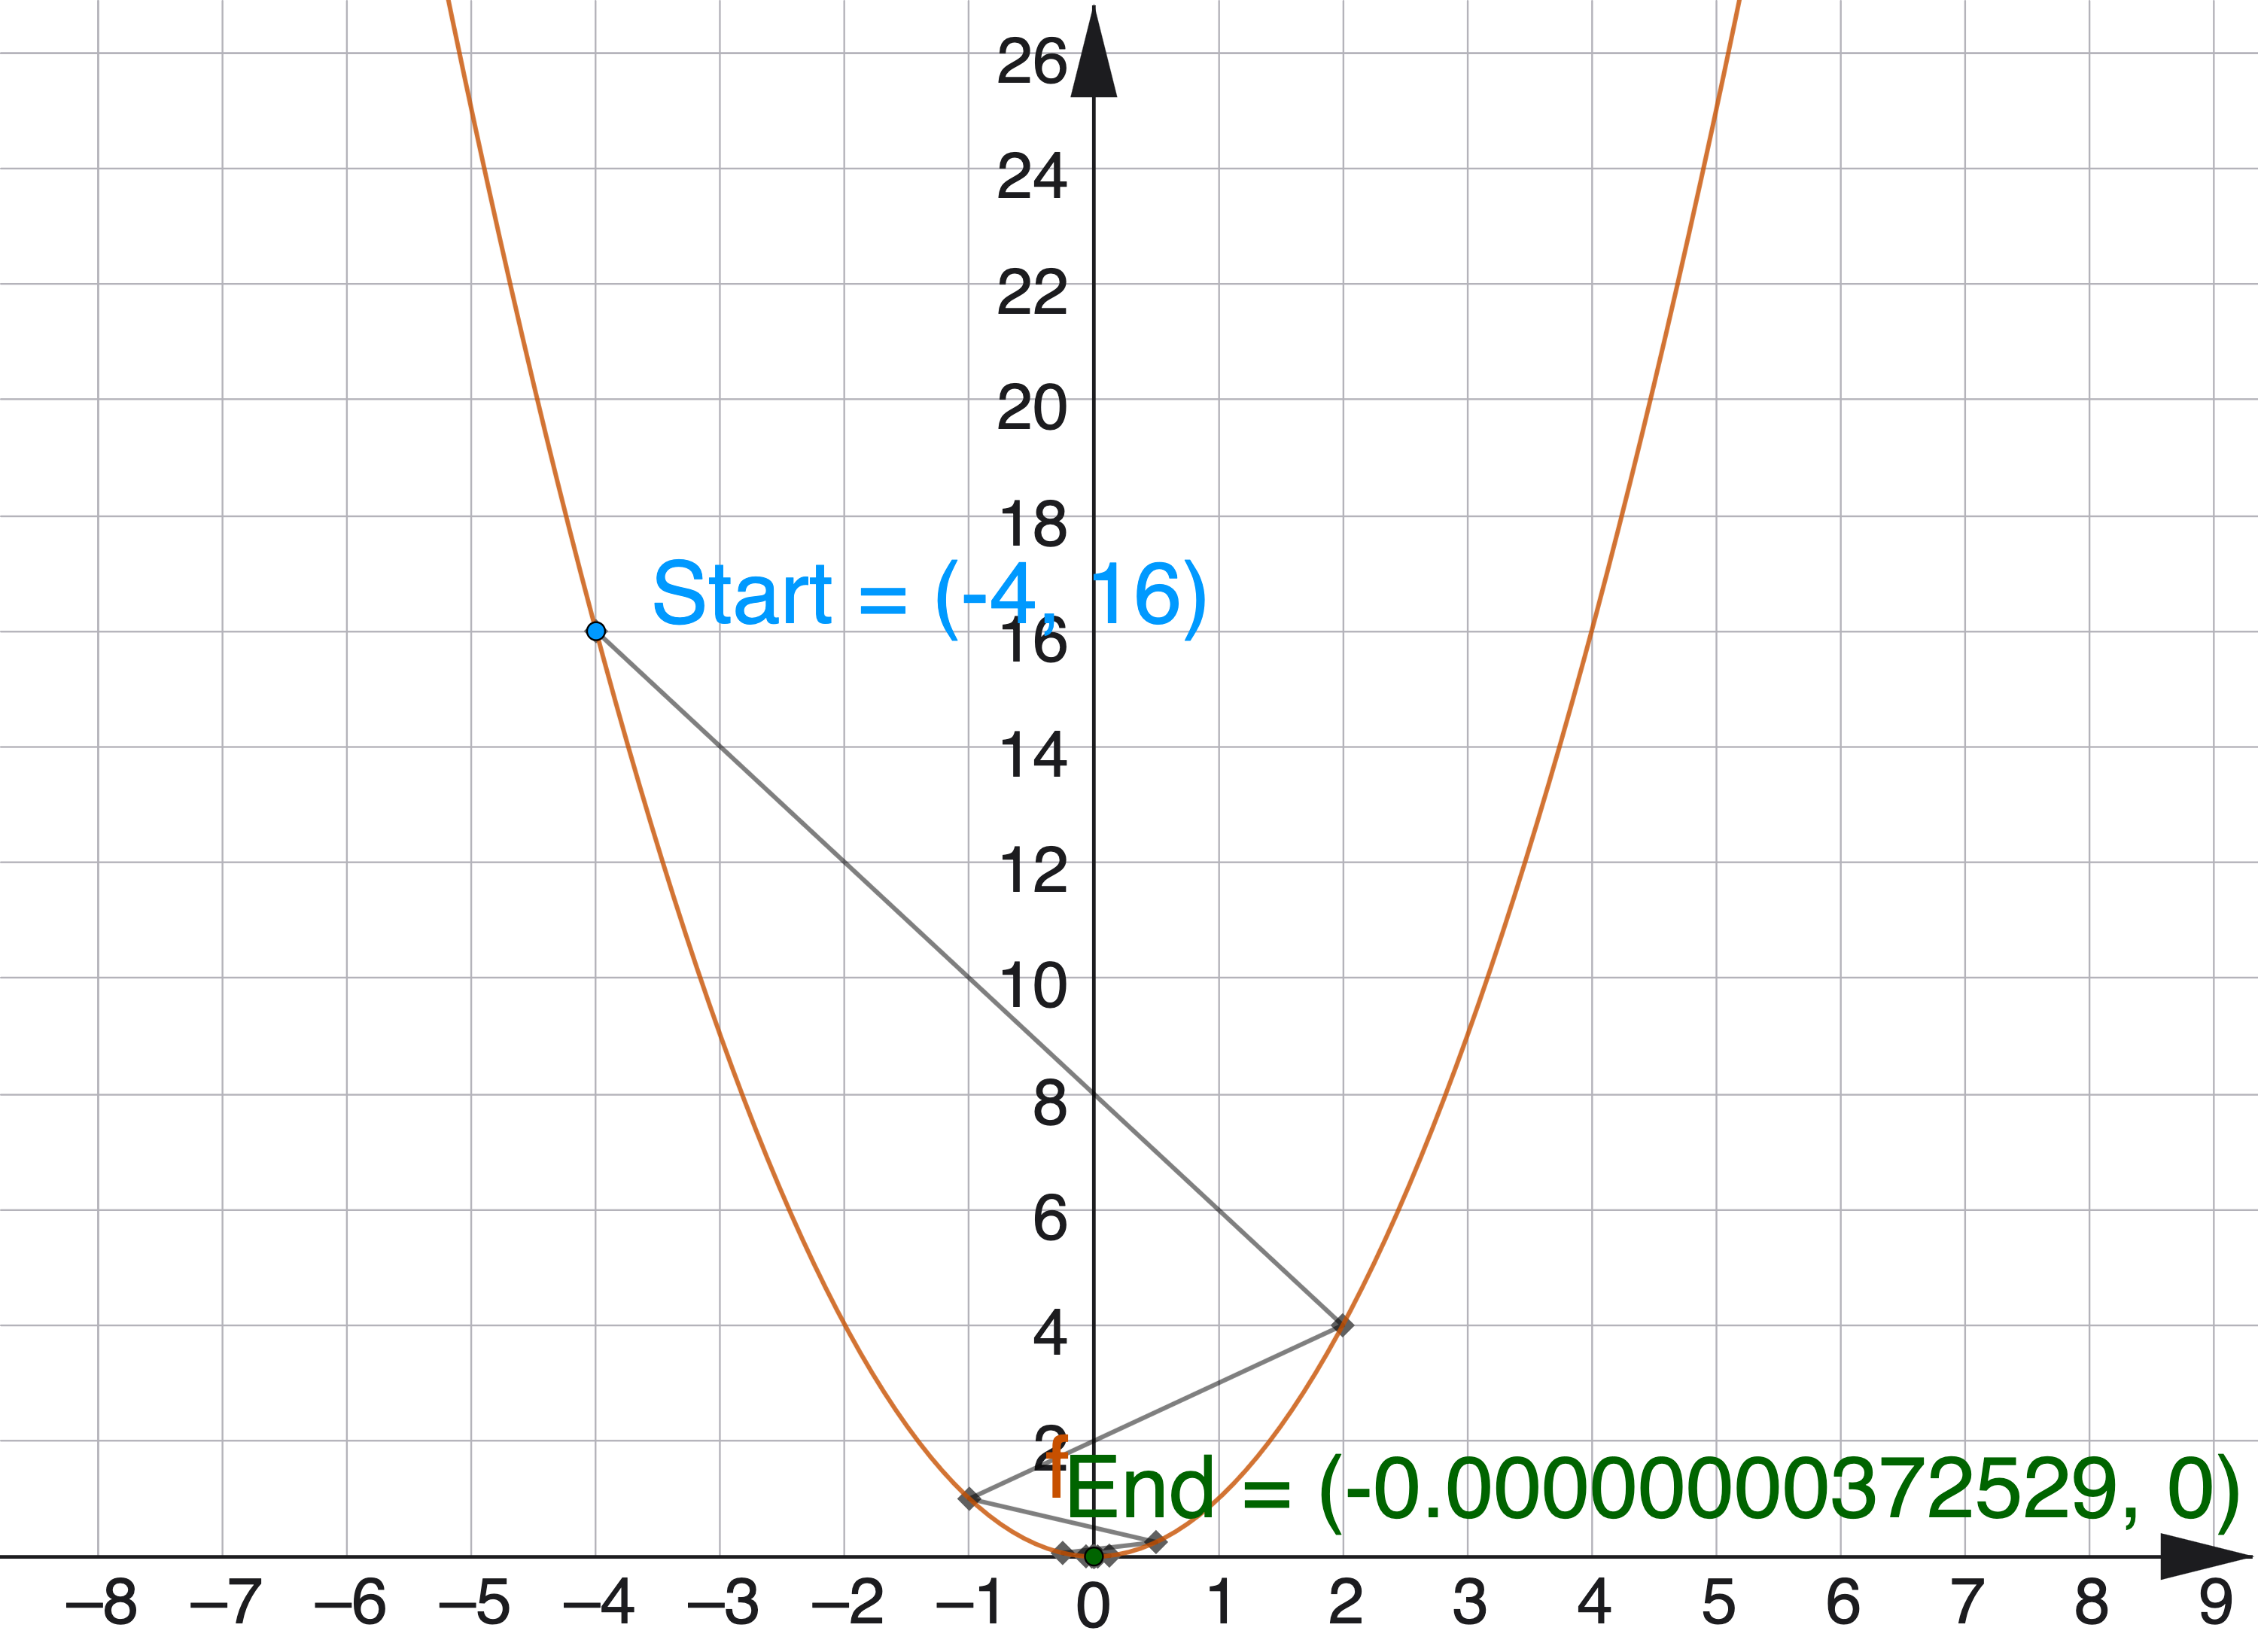
\includegraphics[width=\linewidth]{images/lr_med}}
    \column{0.33\textwidth}
        \centering
        \only<4->{
        $\alpha$ too large:\\divergence
        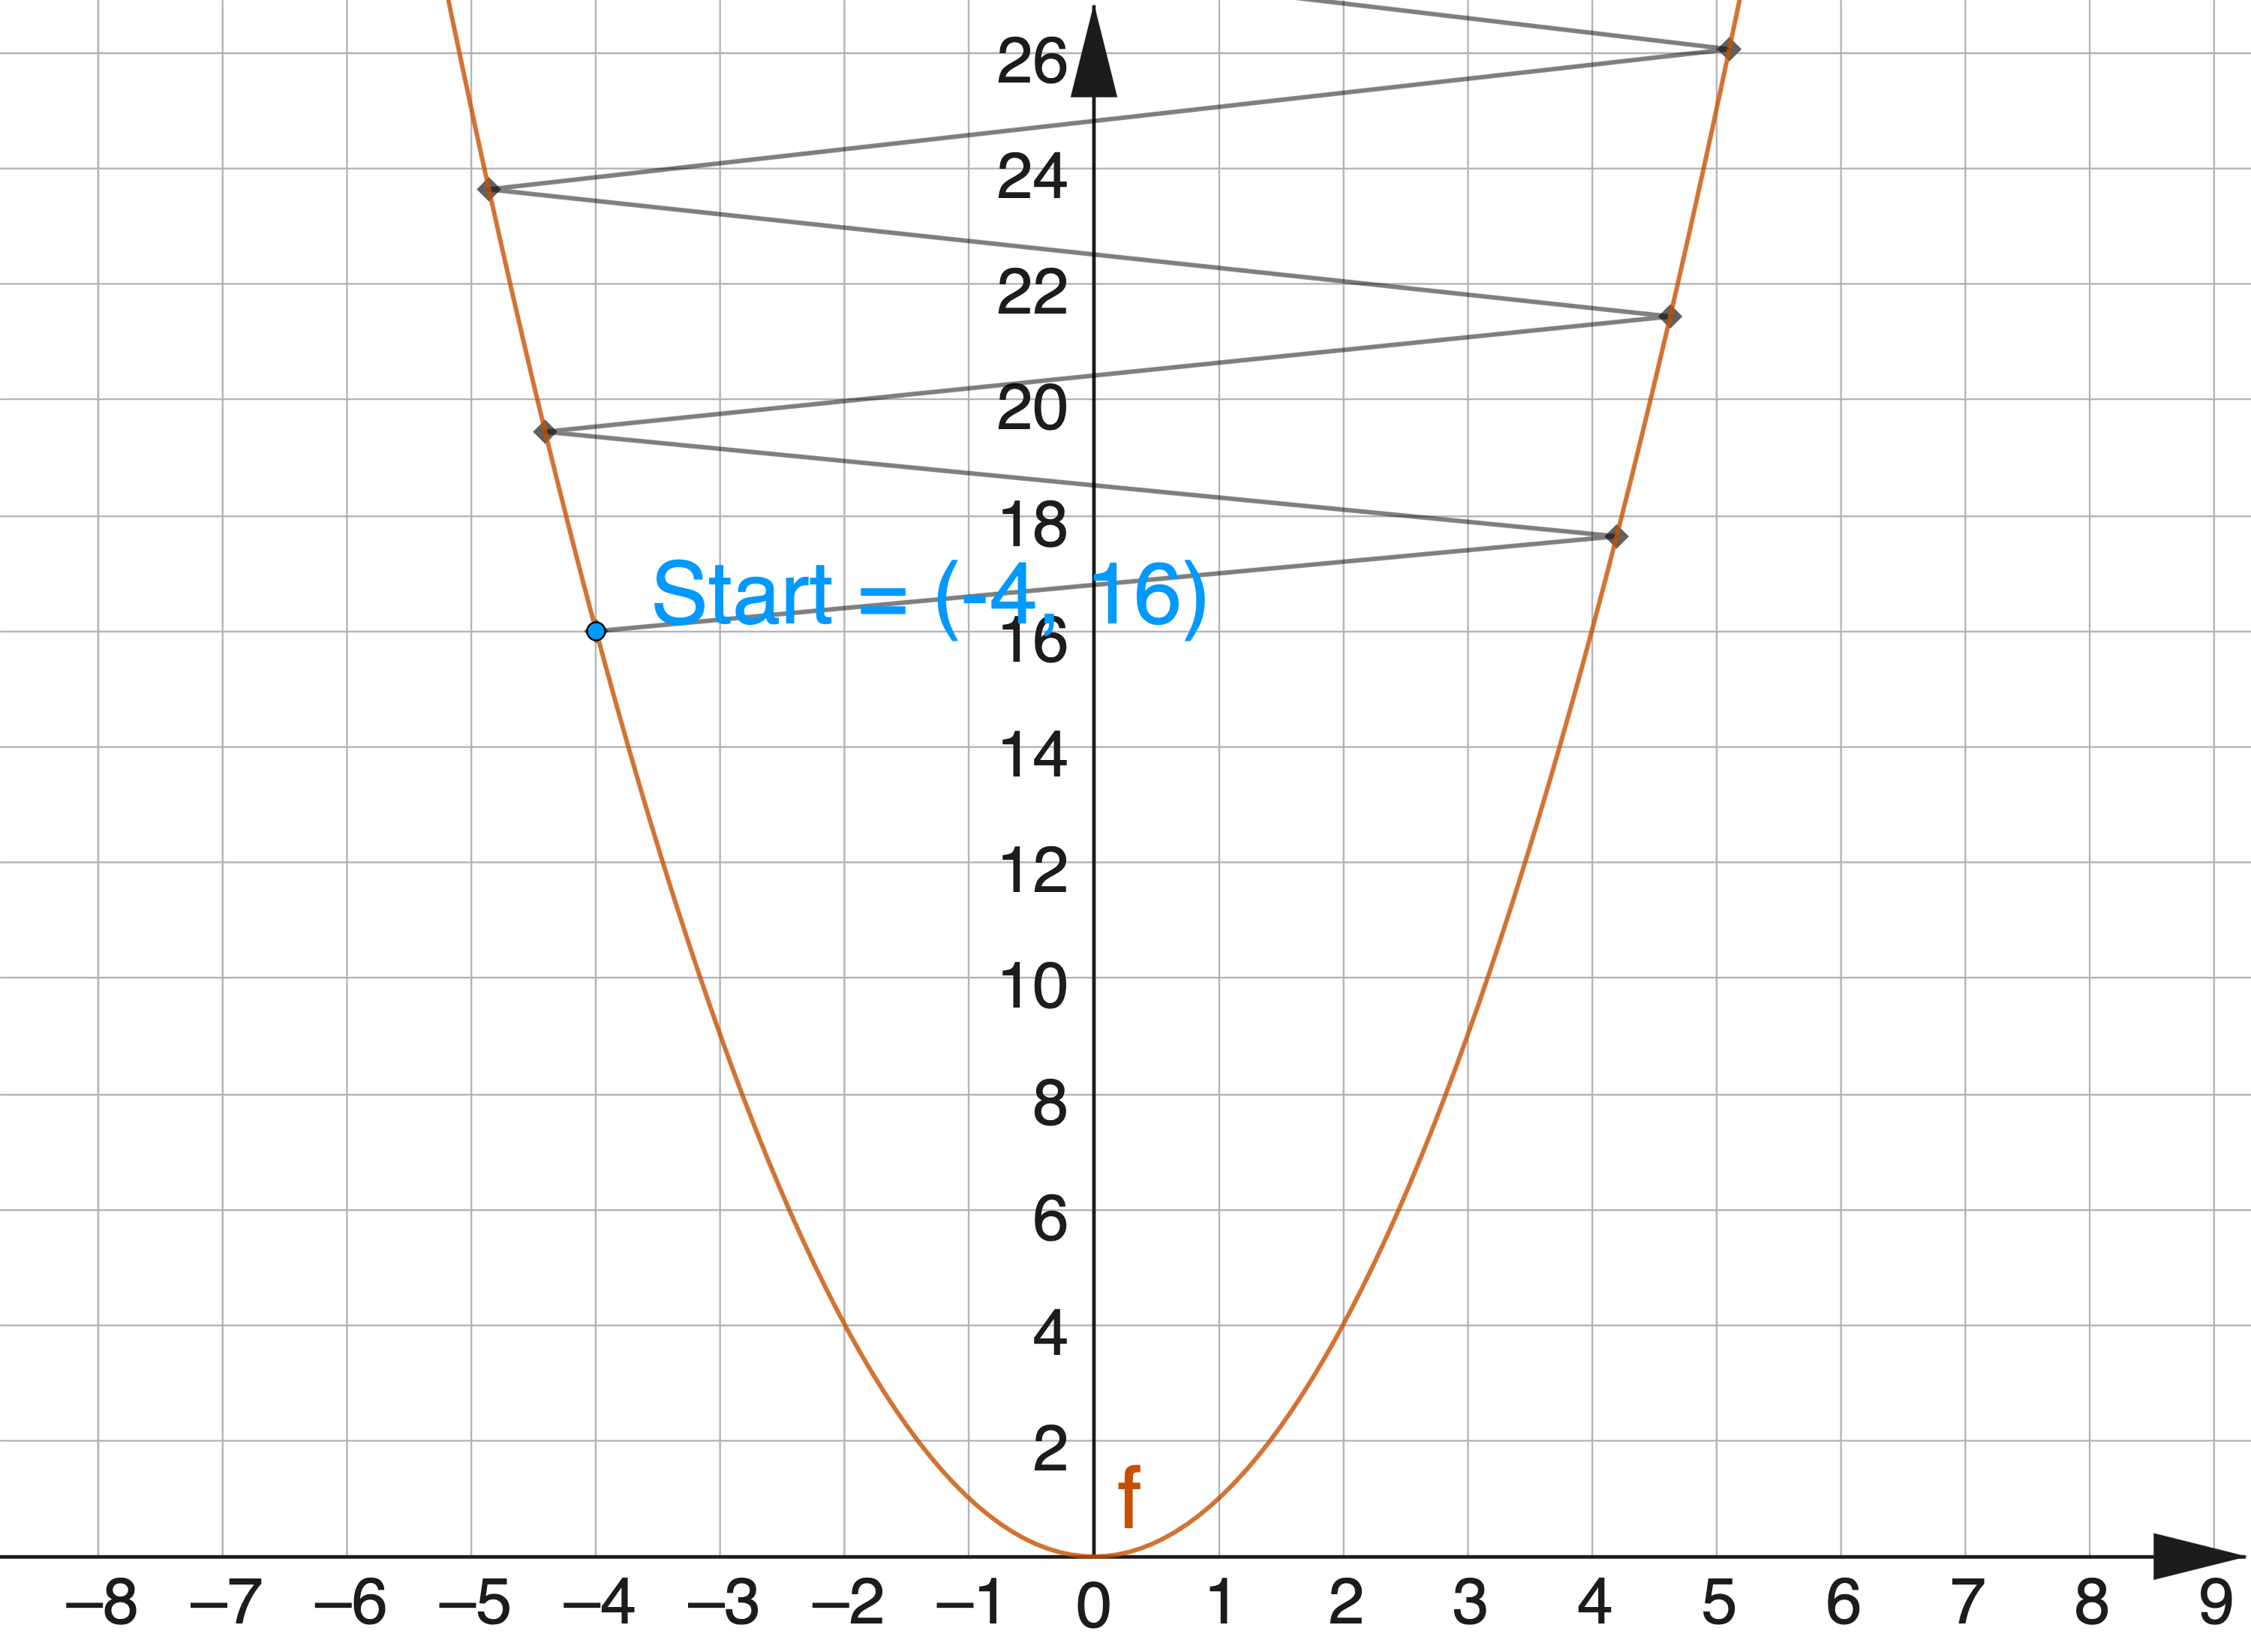
\includegraphics[width=\linewidth]{images/lr_too_large}}
    \end{columns}
    \only<2->{
    \liturl{Interactive GeoGebra Example}{https://www.geogebra.org/calculator/m3mg8qnt}}
\end{frame}
%-----------------------------------------------------------------------
%----------------------------------------------------------------------
\begin{frame}{Example: Learning Rates in Deep Learning}
    Fixed learning rates are not a good idea in practice!
    \vspace{2ex}
    \begin{columns}
    \column{0.5\textwidth}
        \centering
        $\alpha$ static\\
        (0.9285301)
        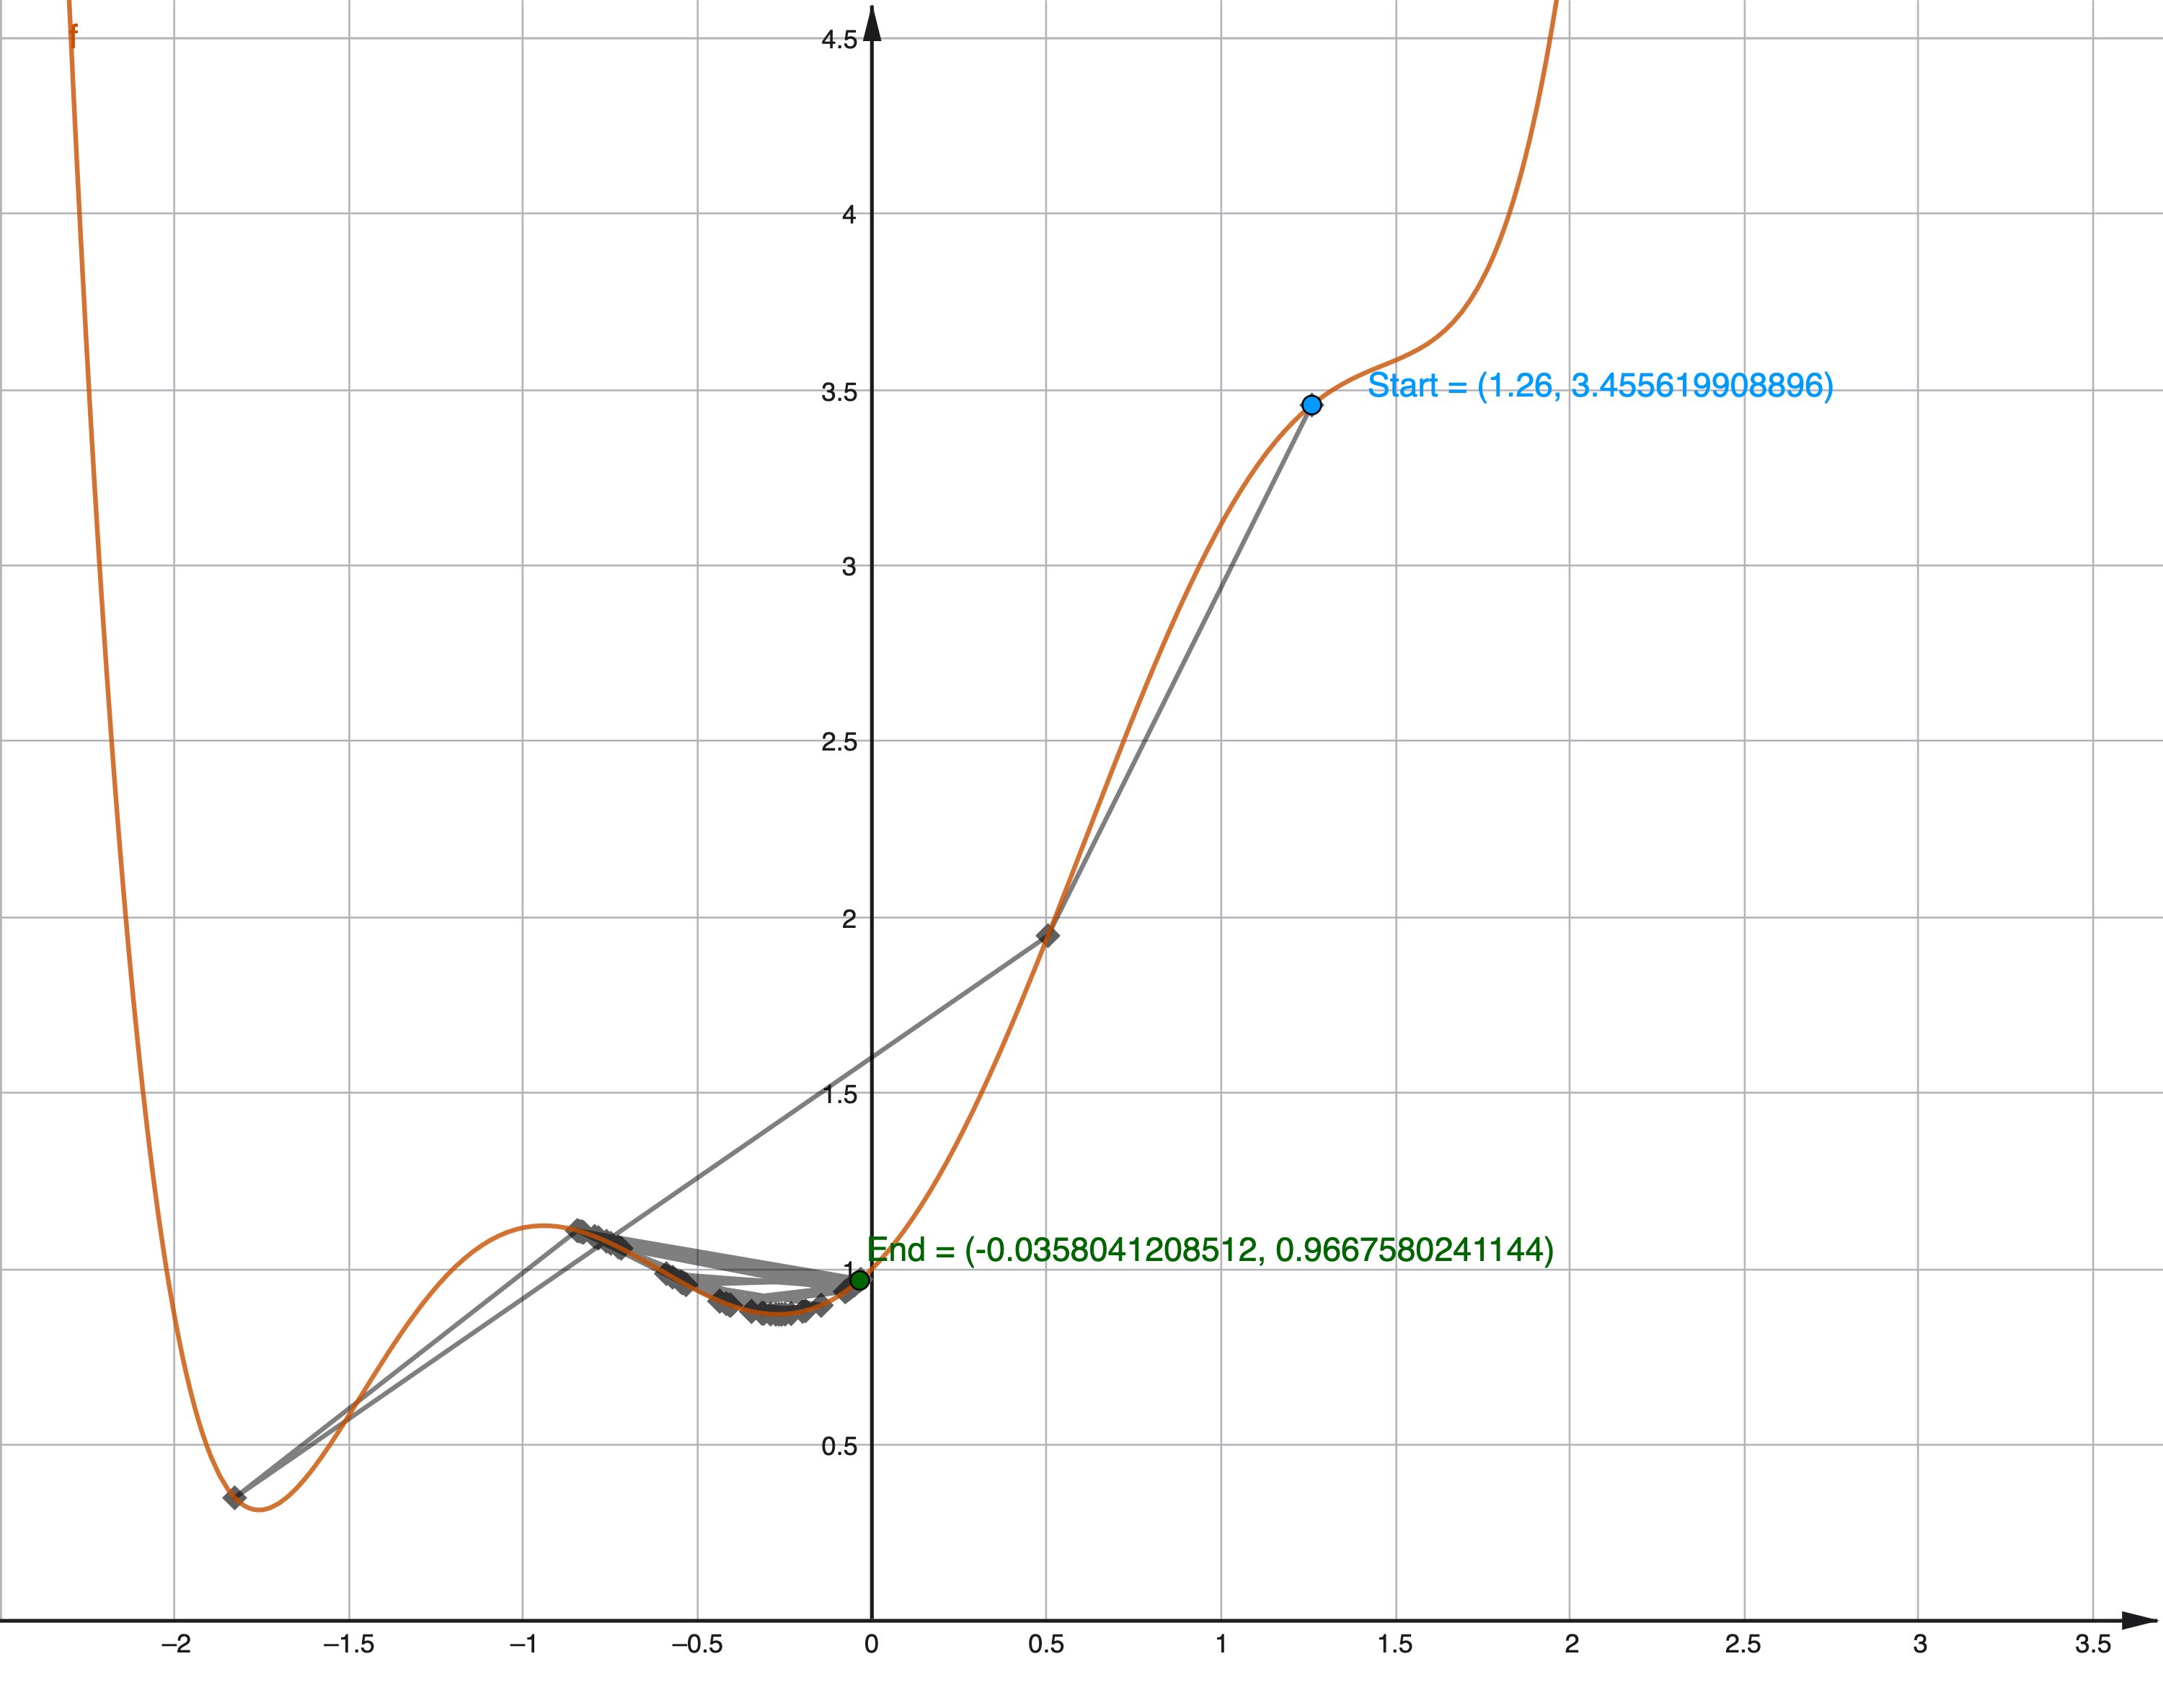
\includegraphics[width=.75\linewidth]{images/ThreeHumpCamle_static_lr.png}
    \column{0.5\textwidth}
        \only<2->{
            \centering
            $\alpha$ manually changed after 3 steps\\(from 0.9285301 to 0.1428201)
            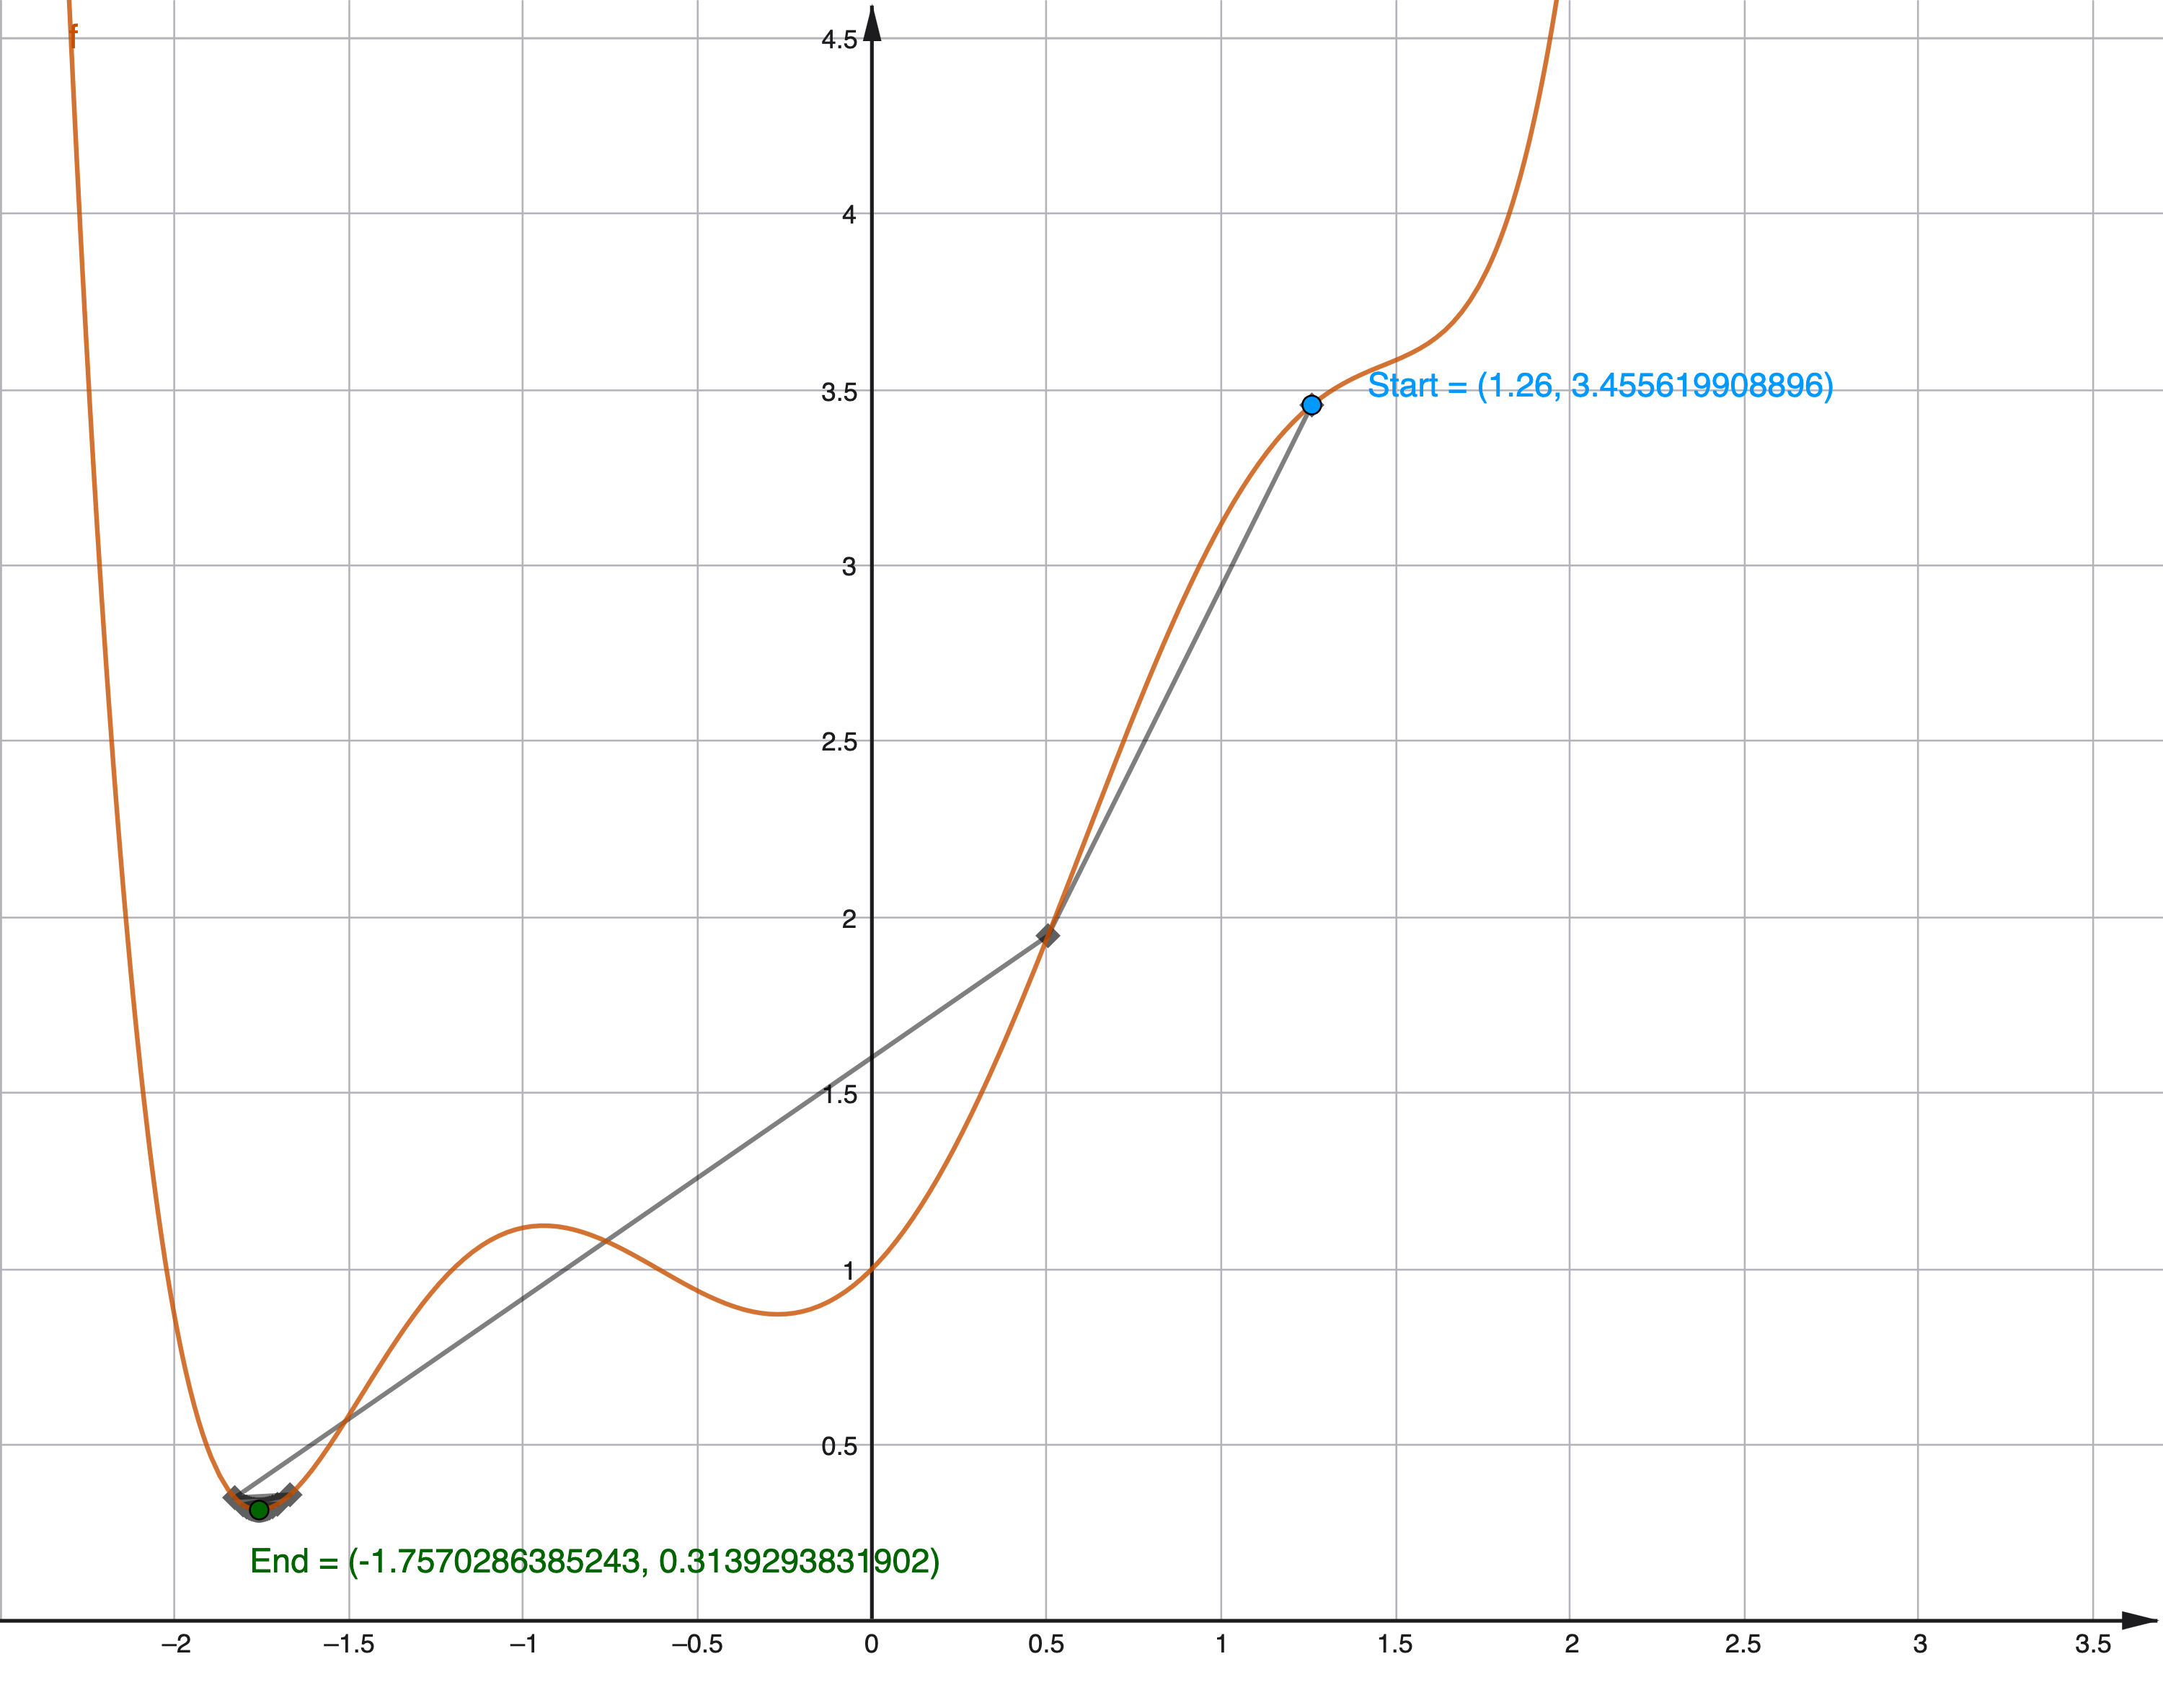
\includegraphics[width=.75\linewidth]{images/ThreeHumpCamel_dynamic}
        }
    \end{columns}
    \liturl{Interactive GeoGebra Example}{https://www.geogebra.org/calculator/q5cjdkff}
\end{frame}

%-----------------------------------------------------------------------
%----------------------------------------------------------------------
\begin{frame}{Heuristics} 
Simple rules of thumb.
For example:
\begin{itemize}
    \item Learning rates should decay over time \liturl{Moulines \& Bach, 2011}{https://proceedings.neurips.cc/paper/2011/hash/40008b9a5380fcacce3976bf7c08af5b-Abstract.html}
    \item Restart if no progress was achieved \liturl{Hansen, 2009}{https://dl.acm.org/doi/10.1145/1570256.1570333}\liturl{Loshchilov and Hutter, 2016}{https://arxiv.org/abs/1608.03983}
    \item Explore at the beginning, exploit at the end
\end{itemize}

\end{frame}

%-----------------------------------------------------------------------
%----------------------------------------------------------------------
\begin{frame}{Heuristics} 
Learning Rates example:
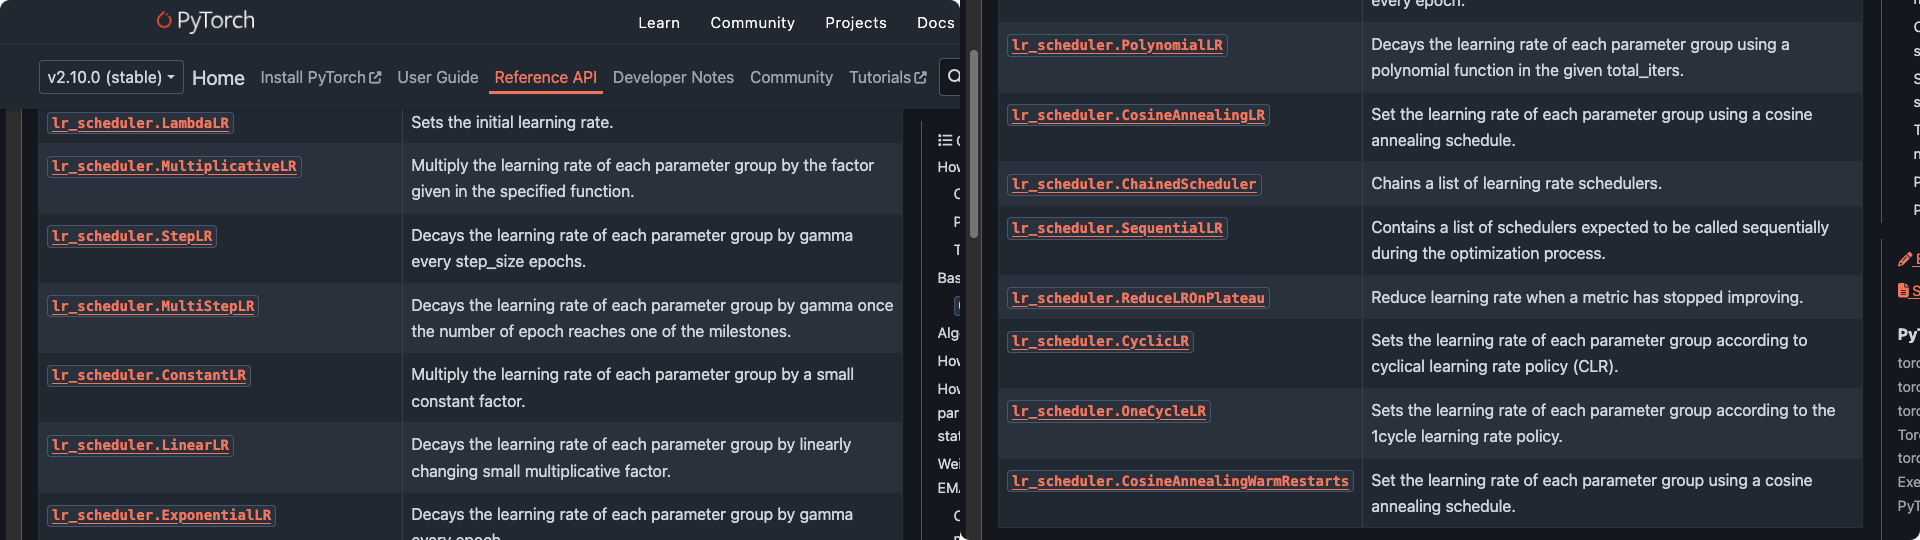
\includegraphics[width=1.0\textwidth]{images/pytorchlrscheds.png}
\liturl{PyTorch v2.10.0 Docs}{https://docs.pytorch.org/docs/stable/optim.html\#how-to-adjust-learning-rate}

\end{frame}

%-----------------------------------------------------------------------
%----------------------------------------------------------------------
\begin{frame}{Schedules/Heuristics Come With Their Own Hyperparameters} 
    \begin{columns}
    \column{0.5\textwidth}
        \centering
        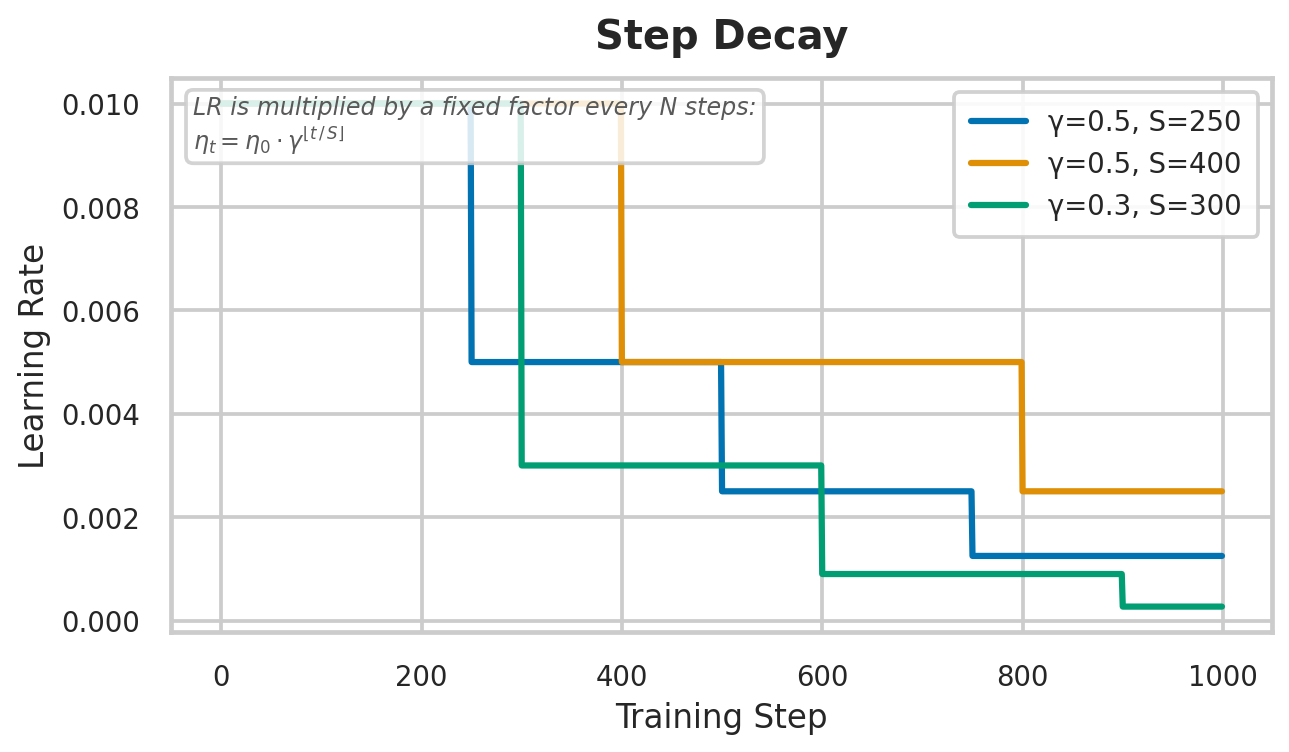
\includegraphics[width=\linewidth]{images/01_step_decay}
        \pause
    %\column{0.33\textwidth}
    %    \centering
    %    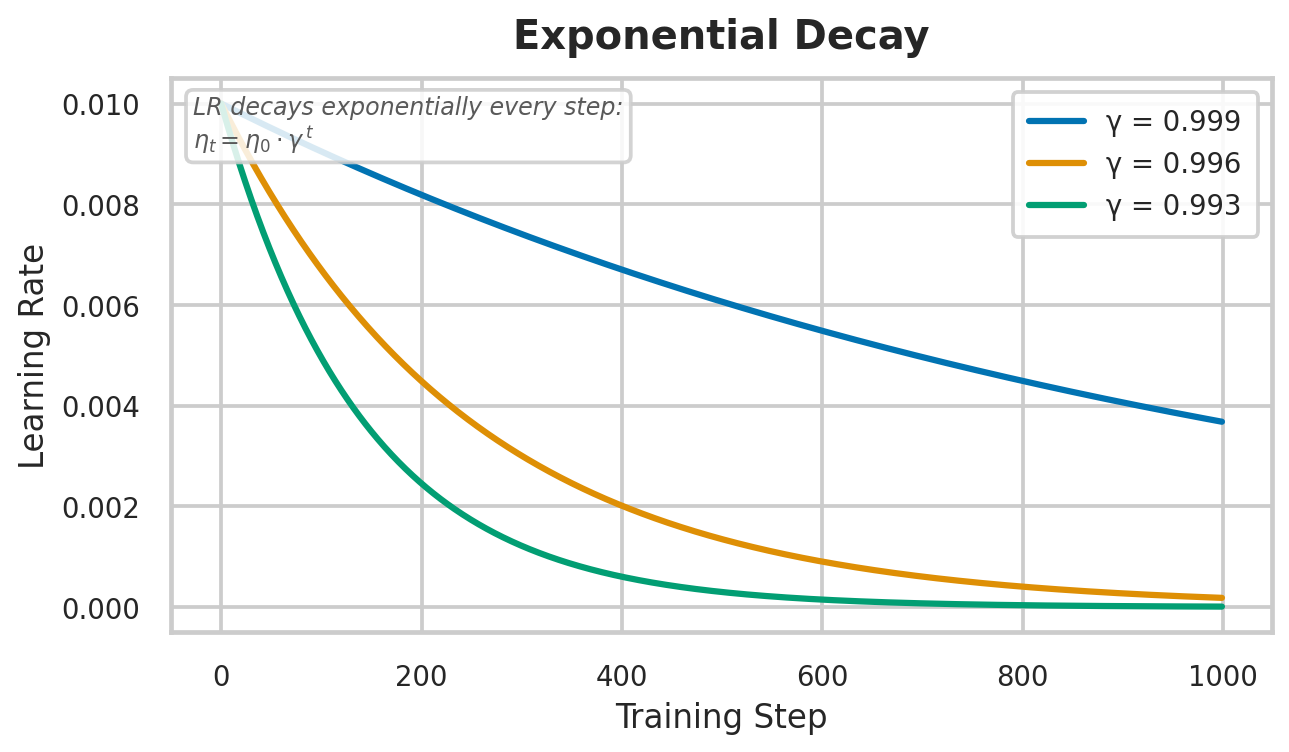
\includegraphics[width=\linewidth]{images/02_exponential_decay}
    %    \pause
    \column{0.5\textwidth}
        \centering
        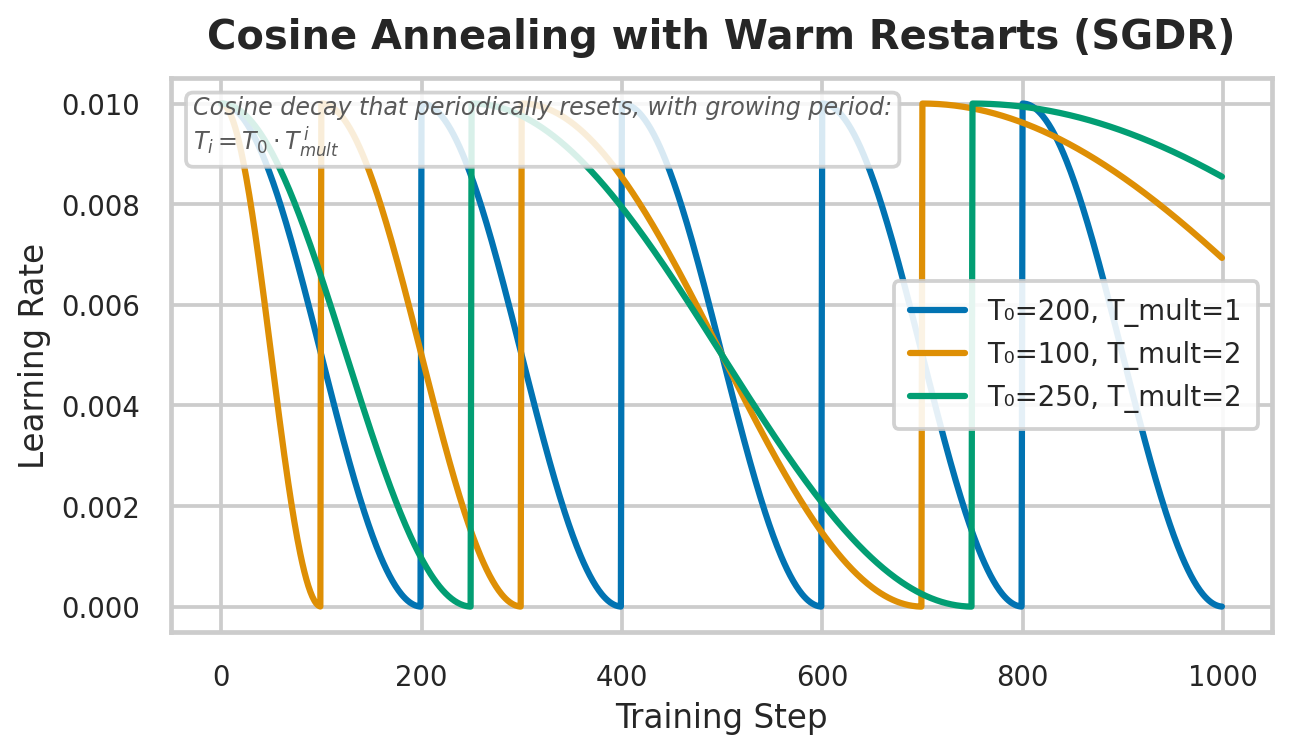
\includegraphics[width=\linewidth]{images/05_cosine_annealing_with_warm_restarts_sgdr}
    \end{columns}
\end{frame}
%-----------------------------------------------------------------------
%----------------------------------------------------------------------
\begin{frame}{Main Takeaways} 

%Most important insights from this video:

\begin{itemize}
    \item \textbf{Learning is often an Iterative Process:} During learning, we traverse a diverse solution landscape. This traversal requires adaptation to the hyperparameters.
    \pause
    \item \textbf{Dynamic Optimization Handles Non-Stationarity:} Changing hyperparameters on-the-fly enables adaptation to the changing solution landscape.
    \pause
    \item \textbf{Community Knowledge:} Heuristics are codified community knowledge that allow for problem specific adaptation via their own hyperparameters. 
\end{itemize}

\end{frame}
%----------------------------------------------------------------------
%----------------------------------------------------------------------

% \begin{frame}[c]{Planning Slide}
% \begin{enumerate}
%     \item Discuss why dynamic is needed
%     \item show examples (e.g. LR, GANs??? as it shows complex interdependencies???)
%     \item show moving landscapes for RL???
%     \item heuristics?
%     \item tuning parameterized schedules?
% \end{enumerate}
% \end{frame}
%-----------------------------------------------------------------------

\end{document}
